\documentclass[10pt,a4paper]{article}
\usepackage[margin=0.95in]{geometry}
\usepackage[utf8]{inputenc}
\usepackage{booktabs}
\usepackage{graphicx}
\usepackage{amsmath,amssymb}
\usepackage{xcolor}
\usepackage{enumitem}
\usepackage{fancyvrb}
\usepackage[font=small,labelfont=bf]{caption}
\usepackage[colorlinks=true,linkcolor=blue!50!black,citecolor=blue!50!black,urlcolor=blue!50!black]{hyperref}
\setlist{itemsep=1pt,topsep=3pt,parsep=0pt}
\setlength{\parskip}{3pt}
\setlength{\parindent}{0pt}
\newcommand{\chem}{\textsc{Chemical}}
\newcommand{\dis}{\textsc{Disease}}

\title{\vspace{-1.2cm}\textbf{Biomedical Named Entity Recognition on BC5CDR:\\
A CRF Baseline with Quantitative and Qualitative Error Analysis}\\[4pt]
\large CS F429 Natural Language Processing --- Project Part 2}
\author{[Group number and member names --- to be filled in before submission]}
\date{October 2026}

\begin{document}
\maketitle
\vspace{-0.8cm}

\begin{abstract}
\noindent We study named entity recognition (NER) for chemicals and diseases in biomedical abstracts using the BC5CDR corpus.
This report covers the classical half of our planned comparison: a feature-based linear-chain Conditional Random Field (CRF)
trained on 5{,}228 training sentences, with regularisation tuned on the development set. The tuned CRF reaches an entity-level
F1 of \textbf{0.8076} on the test set (precision 0.8642, recall 0.7579), versus 0.6787 for a dictionary-lookup baseline.
A detailed error analysis shows that the model is precision-oriented (17.3\% of gold mentions are missed outright, only 6.0\% of predictions are spurious)
and that recall is governed far more by whether an entity string was seen in training (0.498 for unseen strings vs.\ 0.971 for strings seen at least 20 times)
than by entity length. Abbreviations are the hardest surface form (recall 0.461) and account for most chemical/disease type confusions.
These findings motivate the transformer-based model and the rare-entity intervention planned for Part~3.
\end{abstract}

%------------------------------------------------------------------------------------
\section{Introduction}
Biomedical text is growing faster than anyone can read it, and much of the knowledge it contains---which drugs cause which adverse effects,
which compounds treat which conditions---is locked in free text. A first step toward extracting that knowledge is \emph{named entity recognition}:
finding spans of text that mention entities of interest and labelling their type. In this project the entity types are \chem{}
(drugs, compounds, elements) and \dis{} (diseases, symptoms, adverse effects), the two types needed for chemical--induced--disease
relation extraction, which is the downstream task for which the BC5CDR corpus was built \cite{li2016bc5cdr,wei2016cdr}.

Biomedical NER is hard for reasons that overall F1 scores can hide. The vocabulary is open-ended (new compounds are named constantly),
the same concept appears under long names, short names and acronyms (``fulminant hepatic failure'' / ``FHF''), and entity boundaries
involve judgement calls about modifiers (``chronic hepatitis B'' vs.\ ``hepatitis B''). Our overall project asks whether rare and
unusually long entities are recognised much less reliably than common, short ones, and whether a targeted intervention can narrow that gap
without hurting overall performance. The full plan compares a classical CRF with a fine-tuned BioBERT model \cite{lee2020biobert}.

\textbf{Scope of this report (Part 2).} We (i)~prepare and validate the data, (ii)~implement and tune a CRF baseline,
(iii)~define the evaluation protocol, (iv)~report results, and (v)~carry out a quantitative and qualitative error analysis,
including breakdowns by entity frequency and length. We also built a command-line demonstration that extracts chemical and disease mentions from raw text.
The BioBERT model and the novel contribution are Part~3 work; no BioBERT results are claimed here.

%------------------------------------------------------------------------------------
\section{Literature Survey}
\textbf{Why the problem matters.} Chemical and disease mentions are the entry point for literature curation, pharmacovigilance and
drug-repurposing pipelines. The BioCreative~V Chemical-Disease Relation (CDR) challenge made this concrete: participants had to recognise
both entity types in PubMed abstracts and then extract the relations between them \cite{wei2016cdr}. The challenge corpus (BC5CDR) \cite{li2016bc5cdr}
has since become a standard benchmark for biomedical NER.

\textbf{Classical sequence labelling.} Conditional Random Fields \cite{lafferty2001crf} model the conditional probability of a label sequence given the input
and were the dominant approach to biomedical NER for years. Strong systems combined CRFs with rich hand-built orthographic and lexical
features: tmChem \cite{leaman2015tmchem} for chemicals and TaggerOne \cite{leaman2016taggerone}, a semi-Markov model that jointly performs recognition and normalisation,
evaluated on chemical and disease corpora. Their strength is cheap training and strong precision on frequent vocabulary; their weakness is dependence
on surface features that cannot capture the meaning of a name never seen before.

\textbf{Neural and pretrained models.} Bidirectional LSTM-CRF taggers with character-level representations \cite{lample2016neural} removed much of the feature engineering,
and Habibi et~al.\ \cite{habibi2017deep} showed that pretrained word embeddings improve biomedical NER without hand-crafted features.
Transformer encoders \cite{devlin2019bert} changed the picture again: BioBERT \cite{lee2020biobert} continues BERT's pretraining on PubMed abstracts and PMC full text,
SciBERT \cite{beltagy2019scibert} pretrains on scientific text with an in-domain vocabulary, and PubMedBERT \cite{gu2021pubmedbert} argues for pretraining from scratch on PubMed
text. Fine-tuned for NER, such models benefit from subword tokenisation and from knowledge absorbed during pretraining, which is exactly what rare names require.

\textbf{Generalisation to unseen entities.} Augenstein et~al.\ \cite{augenstein2017generalisation} analysed NER generalisation across corpora and entity types and showed that
recognising mentions not seen in training is considerably harder than recognising seen ones, a gap that overall scores obscure. This
is the lens we apply to biomedical NER: the error analysis in Section~\ref{sec:errors} measures the gap directly for our CRF, and Part~3 will test whether it persists for BioBERT.

%------------------------------------------------------------------------------------
\section{Dataset and Preprocessing}
\textbf{Corpus.} BC5CDR \cite{li2016bc5cdr} contains 1{,}500 PubMed abstracts (titles and abstracts) split into 500 training, 500 development and 500 test documents,
manually annotated for \chem{} and \dis{} mentions by trained annotators. It is a good fit for this task: the domain is exactly the one we care about, the annotation is
widely used (so results are comparable to the literature), and two entity types give a genuine multi-class problem. We use the sentence-level, token-tagged
version distributed with T-NER \cite{ushio2021tner} (the \texttt{tner/bc5cdr} data), which stores each sentence as a list of tokens and integer BIO tags.
This version does not retain document boundaries, so all statistics here are per sentence.

\textbf{Preprocessing (implemented in \texttt{data\_pipeline.py}).}
\begin{enumerate}
\item \emph{Label decoding.} Integer tags are mapped to BIO strings using the label map shipped with the data
(\texttt{O}=0, \texttt{B-Chemical}=1, \texttt{B-Disease}=2, \texttt{I-Disease}=3, \texttt{I-Chemical}=4). Example (training sentence 1):
\begin{Verbatim}[fontsize=\footnotesize,xleftmargin=1em]
raw tags : [1, 0, 0, 0, 0, 0, 1, 0]
tokens   : Naloxone reverses the antihypertensive effect of clonidine .
BIO tags : B-Chemical O O O O O B-Chemical O
\end{Verbatim}
\item \emph{Validation.} For every sentence we check that tokens and tags have equal length and that the BIO sequence is well formed
(an \texttt{I-X} tag must follow \texttt{B-X} or \texttt{I-X}). All three splits pass with \textbf{zero} violations.
\item \emph{Normalisation choices.} Tokens are used as provided (the corpus is already tokenised, splitting hyphens and apostrophes into separate tokens).
We deliberately do \emph{not} stem, lower-case destructively or remove stopwords: casing, affixes and digits carry strong signal for chemical and disease names,
so the CRF receives the original token and derives lower-cased and shape features itself (Section~\ref{sec:method}). Raw text given to the demo is tokenised
with the same word/punctuation convention (\texttt{\textbackslash w+|[\textasciicircum\textbackslash w\textbackslash s]}), which we verified matches the corpus convention for hyphens and possessives.
\end{enumerate}

\begin{table}[t]
\centering
\small
\caption{BC5CDR statistics after preprocessing (sentence-level).}
\label{tab:data}
\begin{tabular}{lrrrrrrr}
\toprule
Split & Sent. & Tokens & Tok./sent. & Chem. & Dis. & Mentions & Entity tok. \\
\midrule
Train & 5,228 & 109,322 & 20.9 & 5,203 & 4,182 & 9,385 & 11.5\% \\
Dev & 5,330 & 108,958 & 20.4 & 5,347 & 4,244 & 9,591 & 11.5\% \\
Test & 5,865 & 116,318 & 19.8 & 5,385 & 4,424 & 9,809 & 10.9\% \\
\midrule
Total & 16,423 & 334,598 & -- & 15,935 & 12,850 & 28,785 & -- \\
\bottomrule
\end{tabular}
\end{table}


\textbf{Statistics.} Table~\ref{tab:data} shows that the splits are balanced in size and entity mix, and that only about 11\% of tokens belong to an entity,
so token-level accuracy would be misleadingly high (Section~\ref{sec:metrics}). The mention counts agree with those published for the BC5CDR splits.

\textbf{Limitations and biases.} (i)~\emph{Frequency imbalance and a long tail:} 37.9\% of test mentions are strings never annotated with that type in training,
and a handful of common names account for a large share of mentions. (ii)~\emph{Annotation choices:} generic terms such as ``pain'' or ``death'' are annotated
inconsistently (Section~\ref{sec:errors}), which caps achievable precision. (iii)~\emph{Domain coverage:} abstracts about drug-induced toxicity and
cardiovascular, renal and neurological effects dominate, so results may not transfer to clinical notes or other corpora. (iv)~\emph{Sentence-level format:}
document context (e.g.\ an acronym defined earlier in the abstract) is unavailable to a sentence-level tagger.

%------------------------------------------------------------------------------------
\section{Method: Linear-Chain CRF}\label{sec:method}
\textbf{Model.} We tag each sentence with a linear-chain CRF \cite{lafferty2001crf} over the five BIO labels. Given tokens $x_{1:T}$ and labels $y_{1:T}$,
\begin{equation}
p(y\mid x)=\frac{1}{Z(x)}\exp\Big(\sum_{t=1}^{T}\sum_{k}\lambda_k f_k(y_t,x,t)+\sum_{t=2}^{T}\mu_{y_{t-1},y_t}\Big),
\end{equation}
where $f_k$ are binary or real-valued state features, $\mu$ are label-transition weights and $Z(x)$ normalises over all label sequences.
Training minimises the regularised negative log-likelihood
\begin{equation}
\mathcal{L}(\theta)=-\sum_{i}\log p\big(y^{(i)}\mid x^{(i)}\big)+c_1\lVert\theta\rVert_1+c_2\lVert\theta\rVert_2^2 ,
\end{equation}
using L-BFGS (the orthant-wise variant when $c_1>0$). The $\ell_1$ term drives most weights to exactly zero, so the model is sparse and robust to noisy features;
the $\ell_2$ term controls the magnitude of the remaining weights. Decoding uses Viterbi. We enable \texttt{all\_possible\_transitions}, which lets the model learn negative weights for
label pairs never observed in training (for example \texttt{O}$\rightarrow$\texttt{I-Disease}), so that ill-formed BIO sequences are actively discouraged.

\textbf{Features.} Every token is described by the following attributes, computed for the token itself and for each of its neighbours at offsets $\pm1,\pm2$
(neighbour features are prefixed with the offset), plus a bias term and beginning/end-of-sentence markers:
\begin{center}\small
\begin{tabular}{@{}ll@{}}
\toprule
Group & Attributes \\
\midrule
Lexical & lower-cased word form \\
Affixes & first 2 and 3 characters; last 2 and 3 characters \\
Orthographic & is-all-upper, is-title-case, contains-digit, contains-hyphen \\
Word shape & characters mapped to \texttt{X}/\texttt{x}/\texttt{d} with repeats collapsed (``IL-6'' $\rightarrow$ ``XX-d'') \\
\bottomrule
\end{tabular}
\end{center}
Affix and shape features are what give a CRF any ability to generalise to unseen chemical names (suffixes such as \emph{-mide}, \emph{-statin}, \emph{-one})
and disease names (\emph{-itis}, \emph{-pathy}, \emph{-emia}); they are central to the error analysis below.

\textbf{Training and implementation details.} The CRF is trained only on the training split. We use \texttt{sklearn-crfsuite} 0.5.0 on top of \texttt{python-crfsuite} 0.9.12
(a Python binding of CRFsuite \cite{okazaki2007crfsuite}), Python 3.13, with L-BFGS, at most 100 iterations and \texttt{all\_possible\_transitions=True}.
No pretrained embeddings are used, so nothing is frozen or fine-tuned; all parameters are learned from BC5CDR.
Training is deterministic: re-training reproduced our earlier model byte for byte.
Training takes roughly 20--40 seconds on a single CPU process (36.3\,s in the original tuning run, 21.3\,s in our verification run).
The resulting model has 19{,}700 non-zero state-feature weights and 25 label-transition weights ($5\times5$).

\textbf{Rationale.} A CRF is the classical, pre-transformer reference point for sequence labelling: fast, interpretable, and a fair representative of the
feature-engineering era. Its explicit feature set makes errors easy to attribute, which suits the diagnostic goal of this project.

\textbf{Hyperparameter selection.} We searched $c_1,c_2\in\{0.01,0.1,0.5\}$ (nine models), selected by \emph{development-set} entity F1,
and evaluated on the test set once with the chosen setting ($c_1=0.1$, $c_2=0.01$). Table~\ref{tab:grid} shows that results are fairly flat (dev F1 0.8097--0.8277):
weak regularisation works best, but the choice is not fragile.

\begin{table}[t]
\centering
\small
\caption{Development-set entity F1 for the nine $(c_1,c_2)$ combinations (best in bold).}
\label{tab:grid}
\begin{tabular}{lrrr}
\toprule
 & $c_2=0.01$ & $c_2=0.1$ & $c_2=0.5$ \\
\midrule
$c_1=0.01$ & 0.8267 & 0.8225 & 0.8134 \\
$c_1=0.1$ & \textbf{0.8277} & 0.8251 & 0.8148 \\
$c_1=0.5$ & 0.8217 & 0.8192 & 0.8097 \\
\bottomrule
\end{tabular}
\end{table}


%------------------------------------------------------------------------------------
\section{Experiments}
\subsection{Set-up}
We train on the 5{,}228 training sentences, tune on the 5{,}330 development sentences, and report final numbers on the 5{,}865 test sentences.
The test set was not used for any model-selection decision. Baselines and CRF share the same data and the same evaluation code.
All numbers can be regenerated with the commands in the README (Section~\ref{sec:repro}).

\subsection{Metrics}\label{sec:metrics}
We report \emph{entity-level} precision, recall and F1 under exact match, i.e.\ the CoNLL/\texttt{conlleval} convention \cite{tjong2003conll}: a predicted entity counts as correct only if its
\emph{start, end and type} all match a gold entity. Precision $=TP/(TP+FP)$, recall $=TP/(TP+FN)$, F1 is their harmonic mean; we report micro-averages over all mentions
(the headline number) and per-type scores. We chose this because (i)~it is the standard for BC5CDR and CoNLL-style NER, so numbers are comparable with the literature, and
(ii)~it evaluates what the downstream task needs, namely correctly delimited, correctly typed mentions. \emph{Limitations:} exact match is harsh on boundary disagreements
that annotation guidelines leave genuinely ambiguous (we quantify this below with a lenient overlap measure); token-level accuracy would be uninformative because 89\% of tokens are \texttt{O};
micro-averaging weights frequent entities more, so it can hide poor performance on rare ones, which is why we add frequency and length breakdowns;
and the metric ignores entity normalisation (mapping mentions to ontology identifiers).
We implemented the metric ourselves (\texttt{ner\_metrics.py}) following \texttt{seqeval}'s chunking rules, and verified that it reproduces the per-type scores and supports from our first evaluation exactly.

\subsection{Baselines}
\textbf{Dictionary lookup.} A deliberately naive lower bound: build a lexicon of all 2{,}390 distinct (lower-cased) entity strings in the training set,
and tag every test span that matches, longest match first, with the string's most frequent type. Its recall ceiling equals the share of test mentions seen in training.
\textbf{CRF.} The model of Section~\ref{sec:method}. A fine-tuned BioBERT model \cite{lee2020biobert} is the modern baseline planned for Part~3 and is not evaluated here.

\subsection{Results}
\begin{table}[t]
\centering
\small\setlength{\tabcolsep}{3.6pt}
\caption{Entity-level results (exact span and type match). The CRF is trained on the training split only; hyperparameters were chosen on dev and the test set was used for the final numbers.}
\label{tab:results}
\begin{tabular}{llrrrrrrrrr}
\toprule
 & & \multicolumn{3}{c}{Chemical} & \multicolumn{3}{c}{Disease} & \multicolumn{3}{c}{Overall (micro)} \\
\cmidrule(lr){3-5}\cmidrule(lr){6-8}\cmidrule(lr){9-11}
Model & Split & P & R & F1 & P & R & F1 & P & R & F1 \\
\midrule
Dictionary lookup & test & 0.7389 & 0.6082 & 0.6672 & 0.7719 & 0.6282 & 0.6927 & 0.7537 & 0.6172 & 0.6787 \\
CRF ($c_1{=}0.1,c_2{=}0.01$) & dev & 0.9352 & 0.8309 & 0.8800 & 0.8069 & 0.7217 & 0.7619 & 0.8782 & 0.7826 & 0.8277 \\
CRF ($c_1{=}0.1,c_2{=}0.01$) & test & 0.9194 & 0.7885 & 0.8489 & 0.8002 & 0.7206 & 0.7583 & 0.8642 & 0.7579 & 0.8076 \\
\bottomrule
\end{tabular}
\end{table}


Table~\ref{tab:results} gives the main results. The tuned CRF obtains \textbf{0.8076} test F1, 12.9 points above dictionary lookup (0.6787), so it gains substantially beyond memorisation,
via suffix, shape and context features. Three observations: (i)~the CRF is \emph{precision-oriented}: precision (0.8642) exceeds recall (0.7579) on both types;
(ii)~\chem{} (F1 0.8489) is easier than \dis{} (0.7583): chemical names have distinctive morphology, whereas diseases are more often multi-word and boundary-ambiguous;
(iii)~there is a dev--test gap of 2.0 F1 points (0.8277 vs.\ 0.8076). It is concentrated in unseen entity strings: recall on strings seen in training is almost identical on dev and test (0.923 vs.\ 0.917),
whereas recall on unseen strings is lower on test (0.498 vs.\ 0.539) and the test set contains slightly more of them (37.9\% vs.\ 36.6\% of mentions).
Training is deterministic, so we report a single run; we do not have variance estimates over random seeds.

%------------------------------------------------------------------------------------
\section{Error Analysis}\label{sec:errors}
We analyse the 9{,}809 gold and 8{,}602 predicted test entities. Every gold entity is assigned exactly one outcome: \emph{correct}; \emph{type error} (right span, wrong type);
\emph{boundary error} (overlaps a prediction of the same type but the span differs); \emph{boundary+type}; or \emph{missed} (no overlapping prediction).
Every predicted entity is likewise classed as correct, type error, boundary error, or \emph{spurious} (overlaps no gold entity).
Code: \texttt{error\_analysis.py}; all tables and figures below are generated from its output.

\subsection{Quantitative analysis}
\begin{table}[t]
\centering
\small
\caption{Outcome of every gold entity and every predicted entity on the test set (exact-match taxonomy).}
\label{tab:outcomes}
\begin{tabular}{lrrrr}
\toprule
Outcome & Gold entities & \% of gold & Predicted entities & \% of predicted \\
\midrule
Correct (exact span and type) & 7434 & 75.8 & 7434 & 86.4 \\
Boundary error (same type) & 584 & 6.0 & 559 & 6.5 \\
Boundary + type error & 38 & 0.4 & 36 & 0.4 \\
Type error (right span) & 55 & 0.6 & 55 & 0.6 \\
Missed / spurious (no overlap) & 1698 & 17.3 & 518 & 6.0 \\
\midrule Total & 9809 & 100.0 & 8602 & 100.0 \\
\bottomrule
\end{tabular}
\end{table}


\textbf{Where the errors are.} Table~\ref{tab:outcomes} shows that \emph{misses} dominate: 17.3\% of gold mentions get no overlapping prediction,
against 6.0\% boundary errors and only 0.6\% pure type errors. On the precision side 6.0\% of predictions are spurious and 6.5\% have a wrong boundary.
Relaxing the metric to ``overlaps a gold entity of the same type'' would raise recall from 0.758 to 0.817 and precision from 0.864 to 0.929, so about 6 points of each are
attributable to boundary disagreements alone.
Errors differ by type: for \chem{}, 980 of 1{,}139 non-correct gold mentions are outright misses (boundary errors: 105); for \dis{}, misses (718) and boundary errors (479) are both substantial.
Of all 584 gold boundary errors, 82\% involve diseases. At token level (Figure~\ref{fig:conf}), the dominant confusion is a true entity token predicted as \texttt{O}
(19\% of \texttt{B-Chemical}, 21\% of \texttt{B-Disease}), while confusions between chemical and disease labels are rare (the entity-level confusion is 54 chemicals labelled as diseases and 39 the other way).

\begin{figure}[t]
\centering
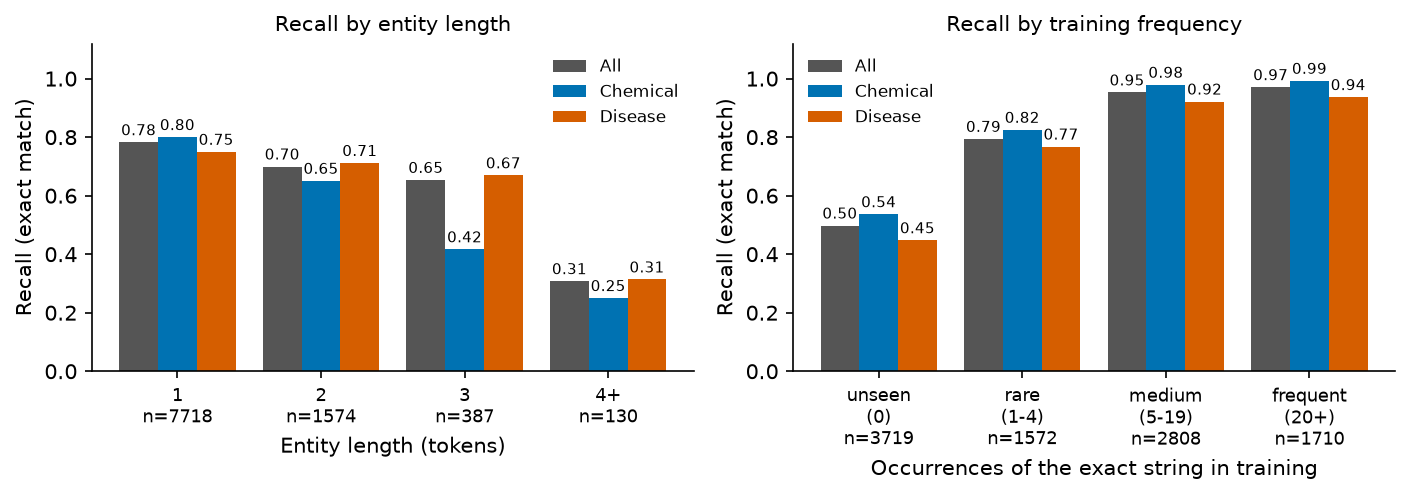
\includegraphics[width=\linewidth]{../figures/recall_by_length_frequency.png}
\caption{Entity-level recall on the test set by entity length (left) and by how often the exact (lower-cased, same-type) string occurs in the training set (right), overall and per type; $n$ is the number of gold mentions.}
\label{fig:lenfreq}
\end{figure}

\textbf{Frequency, not length, is the main driver.} Figure~\ref{fig:lenfreq} (left) shows that recall falls steadily with length: 0.783 for one-token mentions, 0.699 for two, 0.654 for three and only 0.308 for four or more tokens
(precision on predictions of those lengths falls the same way: 0.902, 0.778, 0.688, 0.333). Figure~\ref{fig:lenfreq} (right) shows an even stronger effect of training frequency: recall is 0.498 for the 3{,}719 test mentions (37.9\%) whose exact string never occurs
in training, 0.794 for strings seen 1--4 times, and 0.953 and 0.971 for strings seen 5--19 and 20+ times. Unseen strings account for \textbf{78.7\%} of all non-correct gold mentions.
The two effects are confounded, because long entities are almost never seen before: 126 of the 130 mentions with four or more tokens are unseen. Controlling for this (Table~\ref{tab:lenseen}), recall for
\emph{seen} strings is high at every length (0.92, 0.87, 0.94 for one to three tokens), and for \emph{unseen} strings it is roughly flat at about 0.5 for one to three tokens. The length effect
below three tokens is therefore mostly a frequency effect; only the longest mentions remain disproportionately hard even when unseen (0.286), mostly through boundary errors (59 of the 130 four-plus-token mentions).
For the project's research question this is an important, specific answer: the gap between common and rare entities is large (about 47 points of recall between unseen and frequent strings), and length contributes mainly as a proxy for novelty.

\begin{table}[t]
\centering
\small
\caption{Does length matter once we control for frequency? Recall for seen vs.\ unseen strings.}
\label{tab:lenseen}
\begin{tabular}{lrrrr}
\toprule
Length & Seen: n & Seen: recall & Unseen: n & Unseen: recall \\
\midrule
1 & 5212 & 0.922 & 2506 & 0.492 \\
2 & 734 & 0.873 & 840 & 0.548 \\
3 & 140 & 0.936 & 247 & 0.494 \\
4+ & 4 & 1.000 & 126 & 0.286 \\
\bottomrule
\end{tabular}
\end{table}


\begin{figure}[t]
\centering
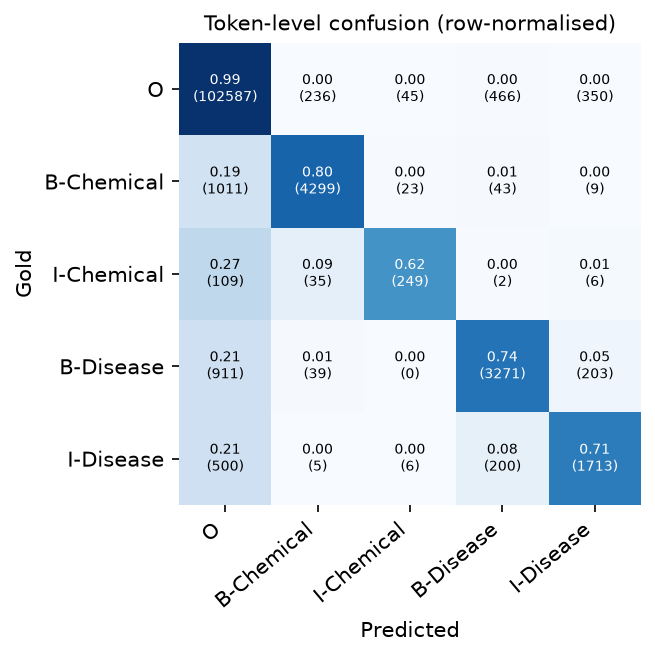
\includegraphics[width=0.52\linewidth]{../figures/token_confusion.png}
\caption{Row-normalised token-level confusion matrix on the test set (counts in parentheses).}
\label{fig:conf}
\end{figure}

\textbf{Surface form.} Table~\ref{tab:surface} (categories are mutually exclusive and assigned in the order listed) shows that \emph{acronyms} are by far the hardest: recall 0.461 on 1{,}148 mentions, with 581 outright misses.
The most frequently missed strings are almost all abbreviations: STZ (18), MI (18), PB (17), CYA (16), APAP (14), CYP (12), GTN (12), plus the unseen drug names diazinon (18) and etomidate (15).
Acronyms are also the main source of type errors, accounting for 33 of the 55. Mentions containing hyphens are comparatively easy (0.842), likely because the hyphen feature and shape features capture them.

\begin{table}[t]
\centering
\small
\caption{Recall by surface form of the gold entity.}
\label{tab:surface}
\begin{tabular}{lrrrrrr}
\toprule
Surface form & Gold & Correct & Recall & Missed & Boundary & Type \\
\midrule
acronym (e.g. ACE) & 1148 & 529 & 0.461 & 581 & 5 & 33 \\
contains digit & 300 & 222 & 0.740 & 58 & 20 & 0 \\
contains hyphen & 240 & 202 & 0.842 & 3 & 26 & 9 \\
multi-word & 1932 & 1292 & 0.669 & 277 & 362 & 1 \\
single plain word & 6189 & 5189 & 0.838 & 779 & 209 & 12 \\
\bottomrule
\end{tabular}
\end{table}


\subsection{Qualitative analysis}
We sampled errors at random (seed fixed; \texttt{results/error\_examples.md} lists 10 per category). Recurring patterns:

\begin{itemize}
\item \textbf{Unseen names with no distinctive morphology are missed.} ``trimethoprim'', ``thyrotropin'', ``clentiazem'', ``diazinon'' and ``subependymal cysts'' are all never seen in training and are not recognised; the
affix features help only when a name looks like others the model has seen. Even seen names are missed when local context is unusual: ``paclitaxel'' (22 training mentions) is missed in ``platinum / paclitaxel - refractory''
because the slash and hyphen disrupt the $\pm2$ window.
\item \textbf{Adjectival and abbreviated disease forms.} ``hypercalcemic'', ``bradycardiac'' and abbreviations such as ``FHF'' (defined as ``fulminant hepatic failure (FHF)'' in the same sentence) are missed; a sentence-level CRF cannot exploit the definition.
\item \textbf{Boundary errors are symmetric and modifier-driven.} The predicted span is too short in 294 cases and too long in 280 (10 shifted). The most frequent pairs (Table~\ref{tab:topbound}) are modifier decisions:
``crack cocaine'' vs.\ ``cocaine'' (11), ``chronic hepatitis B'' vs.\ ``hepatitis B'' (6), ``postoperative delirium'' vs.\ ``delirium'' (5), ``ST depression'' vs.\ ``depression'', ``Renal Toxicity'' vs.\ ``Toxicity''.
Tokenisation also interacts with boundaries: in ``hyper- or hypotension'' the hyphen splits the coordinated mention into two predictions.
\item \textbf{Type errors come from ambiguous abbreviations.} In ``volume of CM administered'' (CM = contrast medium) the model chooses \dis{}; ``MP'' (methylprednisolone), ``TNA'' and the disease abbreviations ``ANT-MI'' and ``XDR-TB''
are mislabelled as the wrong type. The expansion is often given earlier in the abstract, beyond the model's window. Occasionally even an ordinary chemical (``galactose'') is labelled \dis{} in a particular context.
\item \textbf{Spurious predictions: model error and annotation inconsistency.} Of 518 spurious predictions, 222 are \chem{} and 296 \dis{}; 24\% (125) are strings that \emph{are} annotated as an entity at least once in training.
The clearest case is ``death'' (32 spurious predictions): in training it is annotated as a standalone \dis{} in 26 of 32 occurrences, but in the test set in none of 42 (Table~\ref{tab:annprobe}); the model follows the training pattern and is penalised.
Generic symptoms are similarly unstable (``pain'' is annotated in 67\% of its training occurrences but 54\% in test). Other false positives are plausible entities that annotators did not mark (``tachyphylaxis'', ``volume loading'', ``liver enlargement'')
or lexical false cues (``canine'' labelled \chem{}).
\end{itemize}

\begin{table}[t]
\centering
\small
\caption{Most frequent boundary errors (test set).}
\label{tab:topbound}
\begin{tabular}{lllr}
\toprule
Gold & Predicted & Type & Count \\
\midrule
crack cocaine & cocaine & Chemical & 11 \\
sodium chloride & isotonic sodium chloride & Chemical & 7 \\
convulsive & convulsive seizures & Disease & 6 \\
seizures & convulsive seizures & Disease & 6 \\
chronic hepatitis b & hepatitis b & Disease & 6 \\
postoperative delirium & delirium & Disease & 5 \\
hit type ii & hit & Disease & 5 \\
corneal ulcers & ulcers & Disease & 5 \\
downbeat nystagmus & nystagmus & Disease & 5 \\
leukocyturia & sterile leukocyturia & Disease & 5 \\
\bottomrule
\end{tabular}
\end{table}

\begin{table}[t]
\centering
\small
\caption{Annotation consistency probe: how often a string is annotated as a standalone entity (exact span) in training vs.\ test.}
\label{tab:annprobe}
\begin{tabular}{lrrrr}
\toprule
String & Train occurrences & Train annotated & Test occurrences & Test annotated \\
\midrule
death & 32 & 26 & 42 & 0 \\
deaths & 7 & 6 & 7 & 0 \\
pain & 129 & 87 & 83 & 45 \\
hypertension & 67 & 55 & 84 & 63 \\
mi & 0 & 0 & 19 & 19 \\
stz & 0 & 0 & 25 & 25 \\
apap & 0 & 0 & 14 & 14 \\
\bottomrule
\end{tabular}
\end{table}


\subsection{Mitigation}
\begin{itemize}
\item \emph{Unseen vocabulary} (78.7\% of errors): replace word-identity features with representations that carry knowledge of rare names, i.e.\ subword tokenisation and domain pretraining (BioBERT/PubMedBERT-style models), or add gazetteer/ontology features;
a frequency-aware training or augmentation strategy targeted at rare entities is our planned Part~3 contribution.
\item \emph{Abbreviations}: document-level context or an abbreviation-resolution step that propagates the label of a definition (``fulminant hepatic failure (FHF)'') to later uses; contextual encoders with wider windows.
\item \emph{Boundaries}: sequence models with wider context, span-level decoding, and clearer treatment of modifiers; reporting both exact and lenient scores to separate guideline ambiguity from model error.
\item \emph{Annotation noise}: because some ``errors'' reflect inconsistent annotation, we report this analysis alongside the metric rather than treating exact-match F1 as the whole truth.
\end{itemize}

\textbf{Limitations of this analysis.} Frequency is measured by exact lower-cased string match, so morphological variants (``ulcer'' / ``ulcers'') count as different strings and the unseen share is, if anything, overstated;
results come from a single deterministic run on one split; and qualitative examples are a random sample, not an exhaustive review.

%------------------------------------------------------------------------------------
\section{System Demonstration}
\texttt{ner\_cli.py} loads the trained model and extracts chemical and disease mentions from raw text (arguments, files, piped input, or an interactive prompt), printing each mention with its type and character offsets,
and optionally JSON. For example, for ``Patients treated with cisplatin developed nephrotoxicity and hearing loss.'' it returns \chem{}: \emph{cisplatin}; \dis{}: \emph{nephrotoxicity}, \emph{hearing loss}.
It also exposes the failure modes analysed above: for ``Haloperidol was given to control agitation in a patient with Parkinson's disease.'' it finds \emph{Haloperidol} and \emph{agitation} but misses \emph{Parkinson's disease},
even though that string occurs 20 times as a disease in training, and for ``\ldots gastric ulcers'' it returns only ``ulcers''. Training can be re-run live with \texttt{python crf\_baseline.py} (about 25 seconds).

%------------------------------------------------------------------------------------
\section{Conclusion and Next Steps}
A tuned feature-based CRF achieves 0.8076 entity-level F1 on the BC5CDR test set, well above a dictionary baseline (0.6787). The error analysis gives a clear picture of what limits it:
unseen entity strings (78.7\% of errors, recall 0.498 vs.\ 0.971 for frequent strings), abbreviations (recall 0.461), and boundary decisions about modifiers (affecting about 6\% of mentions, mostly diseases).
Length matters mainly because long entities are rarely seen. In Part~3 we will fine-tune BioBERT and compare it with this baseline using the same frequency and length breakdowns,
test whether the rare-entity gap narrows, and design a frequency-aware training or augmentation strategy aimed at the unseen-entity errors identified here.

\section*{Reproducibility}\label{sec:repro}
\begin{Verbatim}[fontsize=\footnotesize]
pip install -r requirements.txt
python data_pipeline.py          # raw -> BIO JSON, validation, statistics
python crf_baseline.py           # train best CRF (c1=0.1, c2=0.01), evaluate, save model (~25 s)
python dictionary_baseline.py    # lookup baseline
python error_analysis.py         # error analysis, figures, tables
python ner_cli.py --demo         # demonstration
\end{Verbatim}

\begin{thebibliography}{99}\small
\bibitem{li2016bc5cdr} J.~Li, Y.~Sun, R.~J. Johnson, D.~Sciaky, C.-H. Wei, R.~Leaman, A.~P. Davis, C.~J. Mattingly, T.~C. Wiegers, and Z.~Lu.
BioCreative~V CDR task corpus: a resource for chemical disease relation extraction. \emph{Database}, 2016:baw068.
\bibitem{wei2016cdr} C.-H. Wei, Y.~Peng, R.~Leaman, A.~P. Davis, C.~J. Mattingly, J.~Li, T.~C. Wiegers, and Z.~Lu.
Assessing the state of the art in biomedical relation extraction: overview of the BioCreative~V chemical-disease relation (CDR) task. \emph{Database}, 2016:baw032.
\bibitem{lafferty2001crf} J.~Lafferty, A.~McCallum, and F.~Pereira. Conditional random fields: probabilistic models for segmenting and labeling sequence data. In \emph{Proc.\ ICML}, 2001.
\bibitem{okazaki2007crfsuite} N.~Okazaki. CRFsuite: a fast implementation of conditional random fields (CRFs), 2007. \url{http://www.chokkan.org/software/crfsuite/}.
\bibitem{leaman2015tmchem} R.~Leaman, C.-H. Wei, and Z.~Lu. tmChem: a high performance approach for chemical named entity recognition and normalization. \emph{Journal of Cheminformatics}, 7(Suppl~1):S3, 2015.
\bibitem{leaman2016taggerone} R.~Leaman and Z.~Lu. TaggerOne: joint named entity recognition and normalization with semi-Markov models. \emph{Bioinformatics}, 32(18):2839--2846, 2016.
\bibitem{lample2016neural} G.~Lample, M.~Ballesteros, S.~Subramanian, K.~Kawakami, and C.~Dyer. Neural architectures for named entity recognition. In \emph{Proc.\ NAACL-HLT}, 2016.
\bibitem{habibi2017deep} M.~Habibi, L.~Weber, M.~Neves, D.~L. Wiegandt, and U.~Leser. Deep learning with word embeddings improves biomedical named entity recognition. \emph{Bioinformatics}, 33(14):i37--i48, 2017.
\bibitem{devlin2019bert} J.~Devlin, M.-W. Chang, K.~Lee, and K.~Toutanova. BERT: pre-training of deep bidirectional transformers for language understanding. In \emph{Proc.\ NAACL-HLT}, 2019.
\bibitem{lee2020biobert} J.~Lee, W.~Yoon, S.~Kim, D.~Kim, S.~Kim, C.~H. So, and J.~Kang. BioBERT: a pre-trained biomedical language representation model for biomedical text mining. \emph{Bioinformatics}, 36(4):1234--1240, 2020.
\bibitem{beltagy2019scibert} I.~Beltagy, K.~Lo, and A.~Cohan. SciBERT: a pretrained language model for scientific text. In \emph{Proc.\ EMNLP-IJCNLP}, 2019.
\bibitem{gu2021pubmedbert} Y.~Gu, R.~Tinn, H.~Cheng, M.~Lucas, N.~Usuyama, X.~Liu, T.~Naumann, J.~Gao, and H.~Poon. Domain-specific language model pretraining for biomedical natural language processing. \emph{ACM Transactions on Computing for Healthcare}, 3(1), 2021. arXiv:2007.15779.
\bibitem{augenstein2017generalisation} I.~Augenstein, L.~Derczynski, and K.~Bontcheva. Generalisation in named entity recognition: a quantitative analysis. \emph{Computer Speech \& Language}, 44:61--83, 2017.
\bibitem{ushio2021tner} A.~Ushio and J.~Camacho-Collados. T-NER: an all-round Python library for transformer-based named entity recognition. In \emph{Proc.\ EACL: System Demonstrations}, 2021.
\bibitem{tjong2003conll} E.~F. Tjong Kim Sang and F.~De Meulder. Introduction to the CoNLL-2003 shared task: language-independent named entity recognition. In \emph{Proc.\ CoNLL}, 2003.
\end{thebibliography}

\end{document}
